\documentclass[pdf,fyma2]{beamer}

\usepackage[IL2]{fontenc}
\usepackage[utf8]{inputenc}
\usepackage[czech]{babel}
\usepackage{graphicx}
\usepackage{url}
\usepackage{movie15}

\usetheme{CambridgeUS}  %CambridgeUS je název tématu
\usecolortheme{dolphin}   %dolphin je název barevného tématu

\title{Semestrální projekt}
\subtitle{Strojový překlad pomocí umělých neuronových sítí}
\author{Jonáš Holcner}
\institute[VUT FIT]{Vedoucí: Ing. Igor Szőke, Ph.D.}
\date{23.~ledna.~2018}

\begin{document}

\maketitle

\section{Úvod}

\begin{frame}
\frametitle{Cíle na zimní semestr}
    \begin{enumerate}
          \item Nastudovat teorii a zvolit vhodný nástroj pro vývoj překladače
          \item Najít, zvolit a připravit vhodná data pro trénování
          \item Vytvořit, natrénovat a otestovat překladač pro překlad z jednoho do druhého jazyka
    \end{enumerate}
\end{frame}

\section{Data}

\begin{frame}
\frametitle{Datasety}

        \begin{figure}[h]
            \begin{center}
                \begin{tabular}{|c|}
                  \hline
                  exampleDataset.cs\\
                  \hline
                  Ahoj světe. \\
                  Venku prší. \\
                  \vdots \\
                  Farmář jí steak. \\
                  \hline
                \end{tabular}
                $\Longleftrightarrow$
                \begin{tabular}{|c|}
                  \hline
                  exampleDataset.en\\
                  \hline
                  Hello world. \\
                  It's raining outside. \\
                  \vdots \\
                  Farmer eats steak. \\
                  \hline
                \end{tabular}
            \end{center}	
        	
        \end{figure}

        \begin{figure}[H]
            \begin{center}
             \setlength{\fboxsep}{8pt}
                \fbox{Myslíš,\textvisiblespace že\textvisiblespace venku\textvisiblespace prší\textvisiblespace Jano?}
                $\Longrightarrow$
                \setlength{\fboxsep}{8pt}
                \fbox{myslíš\textvisiblespace ,\textvisiblespace že\textvisiblespace venku\textvisiblespace prší\textvisiblespace  Jano\textvisiblespace ?}
            \end{center}
            \caption{Předzpracování - tokenizace a truecasing}
        \end{figure}


\end{frame}



\section{Teorie}
\begin{frame}
\frametitle{Strojový překlad pomocí neuronových sítí}
  \begin{columns}[T]
    \begin{column}{.3\textwidth}

        \begin{itemize}
              \item Překlad po celých sekvencích (seq2seq)
              \item Rekurentní neuronové sítě (LSTM)
              \item Word embeddings
        \end{itemize}

    \end{column}

    \begin{column}{.8\textwidth}
        \begin{figure}[T]
            \scalebox{0.31}{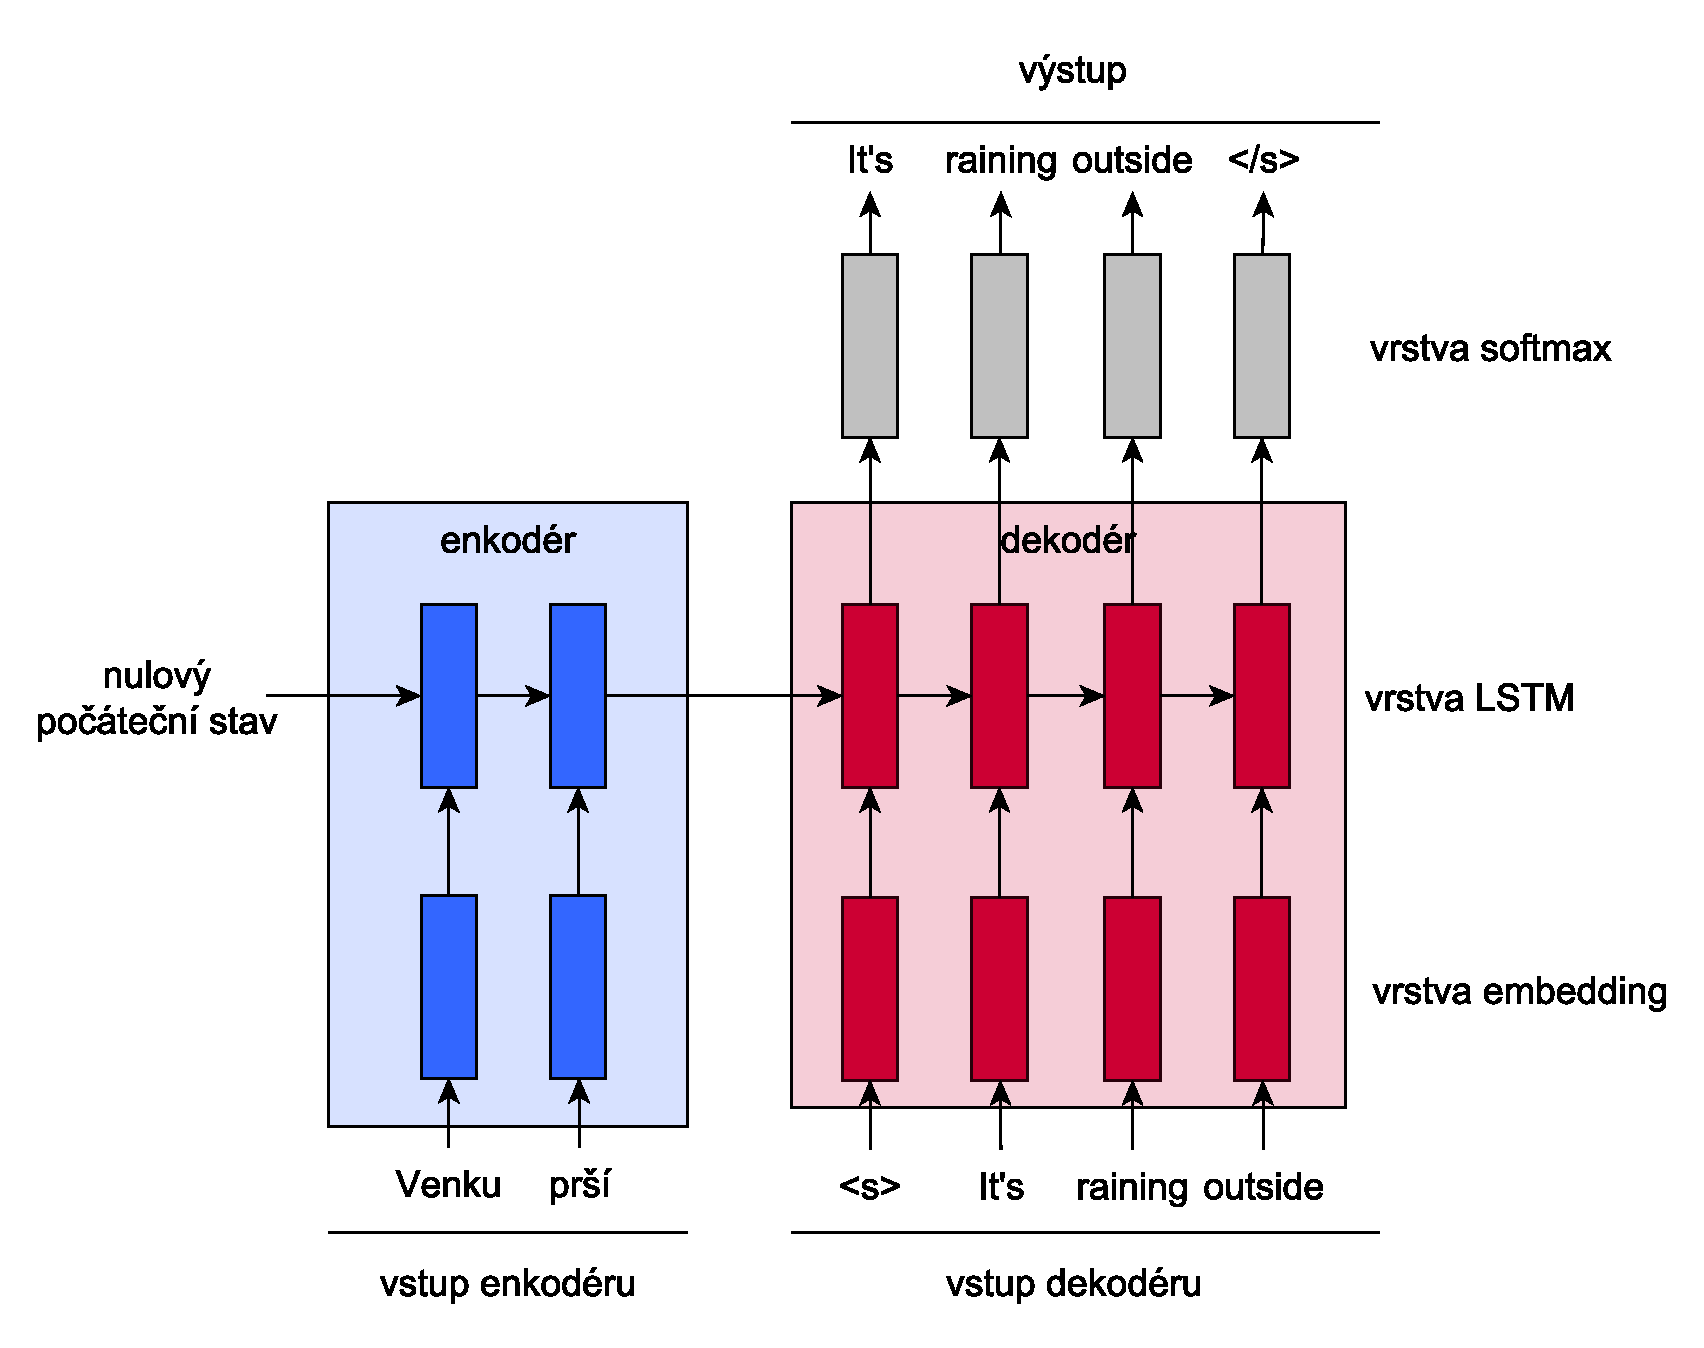
\includegraphics{seq2seq.pdf}}
        \end{figure}
    \end{column}

  \end{columns}
\end{frame}


\section{Co je hotovo}

\begin{frame}
\frametitle{Co jsem udělal}
        \begin{itemize}
            \item Dataset WMT newsCommentary2012 pro trénink, WMT newsTest2017 pro testování. Předzpracování pomocí skriptů z Moses
            \item CS $\Rightarrow$ EN
            \item Baseline systém v nástroji pro statistický překlad Moses
            \item Překladový systém (balíček \emph{nmt} v Python + Keras)
    \item bit.do/pythonNmt
        \end{itemize}
\end{frame}


\begin{frame}
\frametitle{Výsledky}
  \begin{columns}[T]
    \begin{column}{1.0\textwidth}

        \begin{figure}[h]
            \begin{center}
                \begin{tabular}{c|c|c}
                  & baseline v Moses & vytvořený systém \\
                  \hline
                  BLEU skóre & 14.0 & 2.03\\
                  \hline
                \end{tabular}
            \end{center}
        	\caption{Porovnání pro dataset WMT newtest2017 CS $\Rightarrow$ EN}
        	\label{table:results}
        \end{figure}

        \begin{figure}
            \begin{center}
                osmadvacetiletý šéfkuchař nalezen mrtev v obchodě v San Francisku \\ $\Downarrow$ \\
                \_UNK \_UNK \_UNK \_UNK in \_UNK in China
            \end{center}
        	\caption{Ukázka překladu z testovacího datasetu WMT newtest2017}
        \end{figure}

    \end{column}

  \end{columns}
\end{frame}


\section{Závěr}

\begin{frame}
\frametitle{Plán na letní semestr}

     \begin{itemize}
        \item Natrénovat síť přes několik jazyků najednou
        \item Při tokenizaci místo celých slov použít části slov (BPE)
        \item Použít větší datasety (titulky)
        \item Přidat více vrstev RNN a obousměrný enkodér
        \item Použit jinou techniku pro výběr slov při generování (beam search místo greedy search)
    \end{itemize}
    
\end{frame}


\end{document}


